\documentclass[PICOReport.tex]{subfiles}

\begin{document}

%To cover: Galaxy Formation, Clusters, Reionization, point sources (probably moves to a new section called 'Legacy Science')

{\bf The Formation of the First Luminous Sources} \hspace{0.1in} \label{luminoussources}  
A few hundred million years after the Big Bang, the neutral hydrogen gas permeating the Universe was reionized by photons emitted by the first luminous sources to have formed.  The nature of these sources and the exact history of this epoch are key missing links in our understanding of structure formation (SO5).  
%(e.g., star-forming galaxies or high-redshift quasars) and the exact history of this epoch are key missing links in our understanding of structure formation.  
% -- were they star-forming galaxies, high-redshift quasars, or x-ray binaries, to name few candidates --
%Various measurements, including \planck 's determination of the optical depth to reionization $\tau = 0.054 \pm 0.007$, have indicated that reionization concluded by $z \approx 6$, but its onset at higher redshift is poorly constrained. PICO will yield a breakthrough in this context via a cosmic-variance-limited measurement of $\tau$, with $\sigma(\tau)=0.002$, which can only be directly measured in large-scale CMB polarization fluctuations (SO5).  The only proven method to date for measuring this signal, which requires exquisite control of systematics and foreground contamination, is a space-based platform. 
% 

The reionization of the Universe imprints multiple signals in the temperature and polarization of the CMB.  In polarization, the most important signature is an enhancement in the $EE$ power spectrum at large angular scales $\ell \simlt 10$ (Fig.~\ref{fig:clbb}). This signal gives a direct measurement of the optical depth to the reionization epoch $\tau$ and thus to the mean redshift of reionization $z_{re}$, with very little degeneracy with other cosmological parameters (Fig.~\ref{fig:ReionizationPICO}).\footnote{The mean redshit to reionization is the redshift when $50$\% of the cosmic volume was reionized.} \planck 's determination of the optical depth to reionization $\tau = 0.054 \pm 0.007\, (1\sigma) $ have indicated that reionization concluded by $z \approx 6$, but the measurement uncertainty leaves many unanswered questions including: were the ionizing sources primarily star-forming galaxies or more exotic sources such as supermassive black holes or annihilating dark matter? What was the mean free path of ionizing photons during this epoch?  What was the efficiency with which such photons were produced by ionizing sources?  What were the masses and environments of the dark matter halos that hosted the sources?  Did the 
reionization epoch extend to $z \approx 15$-$20$, as has been claimed recently?~\citep{Miranda2017}
PICO's cosmic-variance-limited measurement of the large-scale $E$ modes reaching $\sigma(\tau)=0.002$ will settle these questions. 
\comor{will it settle? or `will significantly constrain the range of candidate models'}. 

%(SO5, and Figure~\ref{fig:ReionizationPICO}) 

Figure~\ref{fig:ReionizationPICO} presents forecasts for reionization constraints in the $z_{re} - \Delta z_{re}$ parameter space. These are obtained from PICO's measurement of $\tau$ in combination with \comor{Stage-III experiments} measurements of the ``patchy'' kinematic Sunyaev-Zel$^{\prime}$dovich (kSZ) effect, due to the peculiar velocities of free electron bubbles around ionizing sources~\citep{Calabrese2014}.
The figure includes curves of constant efficiency of production of ionizing photons in the sources, and of intergalactic-medium opacity, two parameters that quantify models of reionization. The curves shown are illustrative; families of models, that would be represented by parallel \lq source efficiency\rq~and \lq IGM Opacity\rq~lines, are allowed by current data. PICO's data will give simultaneous constraints on these physical parameters, yielding important information on the nature of the first luminous sources. For example, galaxies and quasars predict significantly different values for their IGM opacities and source efficiencies.  

\begin{figure}
\hspace{-0.2in}
\parbox{3.1in}{\centerline {
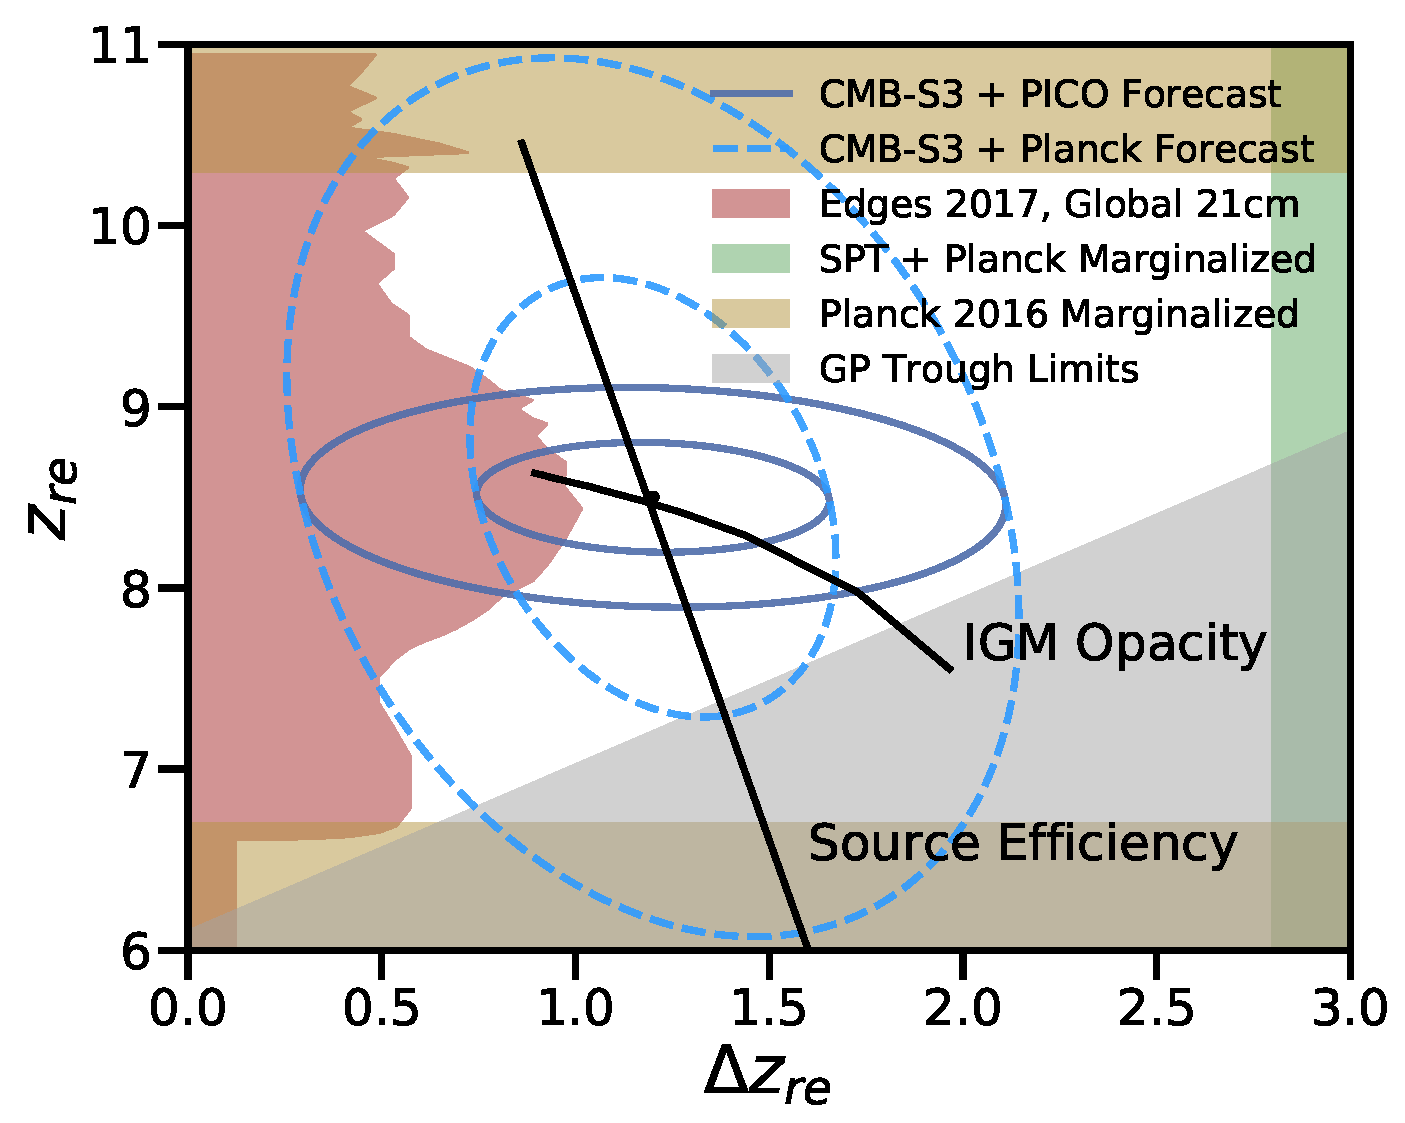
\includegraphics[width=3.0in]{images/Reionization_Contours_zbar_delz_PICO_NEW.pdf} } }
\hspace{0.in}
\parbox{3.5in}{
\caption{\captiontext 
Contours of 1 and 2$\sigma$ constraints on the mean redshift and duration of reionization using PICO and CMB-S3 data (solid dark blue), and comparison with \planck\ and CMB-S3~(dash light blue). Source efficiency and IGM opacity (dark lines) are two physical parameters controlling the reionization process in current models. The PICO measurements, together with higher resolution data of the kSZ effect, will significantly constrain the range of models allowed. We also include other constraints from \planck , EDGES, the Gunn-Peterson (GP) trough, and \planck + the South Pole Telescope~\citep{Planck2018_VI,EDGES2017,Fan2006,Planck2016_reion}.  
%exclusions by EDGES~{edges2017}The solid black lines illustrate how the IGM opacity and source efficiency model parameters map onto this parameter space. The forecasted PICO constraints are compared to: current exclusion limits for the mean redshift of reionization from Planck, shown by the yellow bands \citealp{planck2018:parameters}; recent exclusion limits from the global 21 cm signal measured by EDGES, shown with the red band \citealp{edges2017}; exclusion limits from measurements of the Gunn-Peterson trough from fully absorbed Lyman$\alpha$ in quasar spectra, shown by the grey band \citealp{Fan2006}; exclusion limit on the duration of reionization from Planck and SPT data, shown by the green band \citealp{planck_reio:2016}.
\label{fig:ReionizationPICO}
} }
\vspace{-0.1in}
\end{figure}

%The measurement will also determine the detailed shape of the low-$\ell$ $EE$ spectrum and will thus give information about the reionization history $d\tau/dz$ itself. For example, it has been claimed (and then debated) that \planck\ data show evidence for an extended tail of reionization out to $z \approx 15$-$20$~\citep{Miranda2017}. The PICO measurement will settle this question.  

%Only a measurement over the largest angular scales PICO will yield a breakthrough in this context via a cosmic-variance-limited measurement of $\tau$, with $\sigma(\tau)=0.002$, which can only be directly measured in large-scale CMB polarization fluctuations (SO5).

%The mean redshift of reionization $z_{re}$ depends sensitively on the nature of the ionizing sources and the physics of reionization.  It is currently unknown whether star-forming galaxies or more exotic sources (such as supermassive black holes) drove the reionization process.  What was the mean free path of ionizing photons during this epoch?  What was the efficiency with which such photons were produced by ionizing sources?  What were the masses and environments of the dark matter halos that hosted the sources?  These properties all affect $z_{re}$. Furthermore, the detailed shape of the low-$\ell$ $E$-mode power spectrum is sensitive to the reionization history itself (i.e., $d\tau/dz$), and will provide information beyond that captured in $\tau$ alone.  For example, it has been claimed (and then debated) that \planck~ data show evidence for an extended tail of reionization out to $z \approx 15$-$20$~\citep{Miranda2017}.  A cosmic-variance-limited measurement of the large-scale $E$ modes, as obtained by PICO, will settle this question.  
%The measurement of $\tau$ constrains the mean redshift of reionization, $z_{re}$ (i.e., when $50$\% of the cosmic volume was reionized), which depends sensitively on the nature of the ionizing sources.  For example, it is currently unknown whether star-forming galaxies or more exotic sources (e.g., supermassive black holes) drove the reionization process.  The PICO constraint on $\tau$ is converted to a constraint on $z_{re}$ in Fig.~\ref{fig:ReionizationPICO}, which is further discussed below.  %\comor{not sure about the comment in the parenthesis. $\tau$ is in the STM to 'distinguish between models that describe the formation of the earliest stars' , but that aspect is not highlighted here ...(??). the paragraph also doesn't reference Fig. 3, should it?} 


%Large-scale $EE$ power spectrum measurements are a unique and crucial observable for many aspects of cosmology, particularly the growth of structure.  If measurements of $\tau$ are not improved beyond the current uncertainties from \planck , inference of several new signals of cosmological physics will be severely hindered.  A canonical example is the inference of the sum of the neutrino masses (Page~\pageref{neutrino_fundamental}), but any cosmological results related to the growth of structure will be affected to some extent, including constraints on dark energy and modified gravity from weak lensing, cluster counts, and similar structure probes.  PICO is the ideal experiment to resolve this issue.  Its noise level and frequency coverage permit a cosmic-variance-limited constraint on $\tau$, i.e., $\sigma(\tau) \approx 0.002$, which we have verified with explicit forecasts including separation of foregrounds. 

% We verify this expectation via an explicit forecast following the methodology described in~\citet{errard_feeney_2015}, assuming PICO measurements of the $TT$, $TE$, $EE$, $BB$, and $\phi\phi$ power spectra, with the latter inferred via the iterative $EB$ estimator.  The polarized dust and synchrotron levels match those measured by {\em Planck}~\citep{PlanckFG2015}, including spatial variations, and are cleaned using a parametric maximum-likelihood approach.  Fitting a $\Lambda$CDM$+r$ model, for both the PICO ``requirements'' and ``CBE'' configurations, we find $\sigma(\tau) = 0.002$.  With the exquisite control of systematics needed for the much smaller primordial $BB$ signal, these are not a concern for $EE$ (and hence $\tau$).

%In temperature, an important imprint of reionization is that sourced at small angular scales by the ``patchy'' kinematic Sunyaev-Zel$^{\prime}$dovich (kSZ) effect, due to the peculiar velocities of free electron bubbles around ionizing sources.  Measurements of the small- scale kSZ power spectrum, with instruments that have higher resolution than PICO, can give constraints on the duration of reionizaiton $\Delta z_{re}$~\citep{Calabrese2014}.
%Figure~\ref{fig:ReionizationPICO} presents forecasts for reionization constraints in the $z_{re} - \Delta z_{re}$ parameter space obtained from PICO's measurement of $\tau$ in combination with ground-based Stage-III CMB experiments measurements of the kSZ power spectrum. The PICO measurement of $\tau$ is essential for breaking degeneracies and allowing simultaneous, precise constraints to be placed on both the mean redshift and duration of reionization. The figure also shows curves of constant efficiency of production of ionizing photons in the sources, and of intergalactic-medium opacity. These are two parameters that quantify models of reionization. The curves shown are illustrative; families of models, that would be represented by parallel \lq source efficiency\rq~and \lq IGM Opacity\rq~lines, are allowed by current data. PICO's data will give simultaneous constraints on these physical parameters, yielding important information on the nature of the first luminous sources. For example, galaxies and quasars predict significantly different values for these parameters.  

%The total kSZ power spectrum receives contributions from both the patchy reionization signal and from late-time sources, such as the intergalactic and intracluster media.  The reionization and late-time signals are expected to have comparable amplitudes~\citep{Shaw2012,MMS2012,Battaglia2013}.  With constraints on the late-time contribution from other information (e.g., cross-correlations), effective small-scale foreground removal, and with the primary CMB $TT$ power spectrum constrained by inference from the $EE$ power spectrum,
%It is possible to extract reionization constraints from the small-scale kSZ power spectrum~\citep{calabrese/etal/2014}.  The most directly constrained quantity is the duration of reionization, $\Delta z_{re}$. %\comor{if pico is not providing kSZ constraints, only S3 does, there is no need to dwell on it at all, I think.  Nick, can you condense this?}


%1 and $2\sigma$ PICO constraints on reionization in combination with ground-based Stage-III CMB experiments (CMB-S3) (solid blue) compared to constraints from \planck~data and observations at other wavelengths. 


The process of reionization leaves specific non-Gaussian signatures in the CMB.  In particular, patchy reionization induces non-trivial 4-point functions in both temperature and polarization~\citep{SmithFerraro2017,DvorkinSmith2009}.  The temperature 4-point function can be used to separate reionization and late-time kSZ contributions.  Combinations of temperature and polarization data can be used to build quadratic estimators for reconstruction of the patchy $\tau$ field, analogous to CMB lensing reconstruction (next Section).  These estimators generally require high angular resolution, but also rely on foreground-cleaned CMB maps.  PICO's data in its high-frequency bands --- which have better than 2~arcmin resolution and cover frequencies that are not suitable for observations from the ground --- will enable these estimators to be robustly applied to high resolution ground-based CMB data, a strong example of ground-space complementarity.  %\comor{if pico is complementarity by {\it only} providing foreground maps at sufficiently high resolution, I think we should move this to the 'complementarity'. It is not a direct science goal or outcome.}
%% JCH: I checked the Smith-Ferraro 4-pt estimator, and PICO does not have sufficient resolution to do this (see Fig. 3 of https://arxiv.org/pdf/1803.07036.pdf )
%
%Thus, while PICO alone may not enable high \ac{SNR} reconstructions,

With ten independent maps of the entire sky, multiple frequency bands and ample sensitivity to remove foregrounds, PICO is uniquely suited to make the low $\ell$ $EE$-spectrum measurements that are needed to elucidate the formation of the first luminous sources. No such measurements have yet been done from the ground. Of the currently operating Stage-III experiments, one is targeting the lowest $EE$ $\ell$ modes~\citep{class}. 

Lowering the uncertainty on $\tau$ is crucial for many cosmological observables of the growth of structure. As discussed in Section~\ref{neutrino_fundamental}, these observables are only sensitive to the combination of $\tau$ and $A_{s}$. PICO's cosmic-variance-limited measurement of $\tau$ will break this degeneracy and thus improve constraints on the sum of neutrino masses, on dark energy and modified gravity from weak lensing, and on cosmological parameters deduced from cluster counts \comor{ and anything else?}.  

%%%%%%%%%%

\vspace{0.1in}
\noindent{\bf Probing Structure Formation via Gravitational Lensing} \hspace{0.1in} \label{gravitationallensing}
Matter between us and the last-scattering surface deflects the path of photons through gravitational lensing, imprinting the 3-dimensional matter distribution across the volume of the Universe onto the CMB maps. The specific quantity being mapped by the data is the projected gravitational potential $\phi$ that is lensing the photons. From the lensing map, which
receives contributions from all redshifts between us and the CMB, with the peak of the distribution at $z \simeq 2$, we infer the angular power spectrum $C_{L}^{\phi \phi}$ (Fig.~\ref{fig:lensingNoisePICO}). %, which depends on cosmological parameters \comor{why do we say that it depends on cosmological parameters? is that meant to connect to something later?}.
Both the temperature and polarization maps of the CMB, and by extension the angular power spectra, are affected by lensing. 

\planck 's $\phi$ map had \ac{SNR} of $\sim$1 per $L$ mode over a narrow range of scales, $30 < L < 50$. PICO's map would represent true mapping, with \ac{SNR} $\gg1$ per each mode down to scales of approximately ten arcminutes ($L\footnote{We use $L$ to refer to multipoles in the CMB lensing and galaxy clustering fields, in contrast to the use of $\ell$  for the CMB itself. } \sim 1000$).  On smaller scales, the map will still contain statistical information. While \planck~  had an \ac{SNR} of 40 integrated across the entire $C_{L}^{\phi \phi}$ power spectrum~\citep{2018arXiv180706210P}, the PICO combination of resolution, sensitivity, and sky coverage enables a measurement with SNR of 638 and 737 for the baseline and CBE configurations, respectively.  When accounting for possible foreground contamination, its broad frequency coverage leads to a reduction of SNR of less than 20\% (Fig.~\ref{fig:lensingNoisePICO}).  
% say something about "the best measurement"...?

% Fig.~\ref{fig:lensingNoisePICO} shows per-mode noise curves for the reconstruction of CMB lensing from PICO, demonstrating the wide range of angular scales over which the matter density field will be  mapped.  \textbf{Add brief discussion of foreground robustness demonstrated in Fig.~\ref{fig:lensingNoisePICO}}

\begin{figure}
\hspace{-0.2in}
\parbox{3.0in}{\centerline {
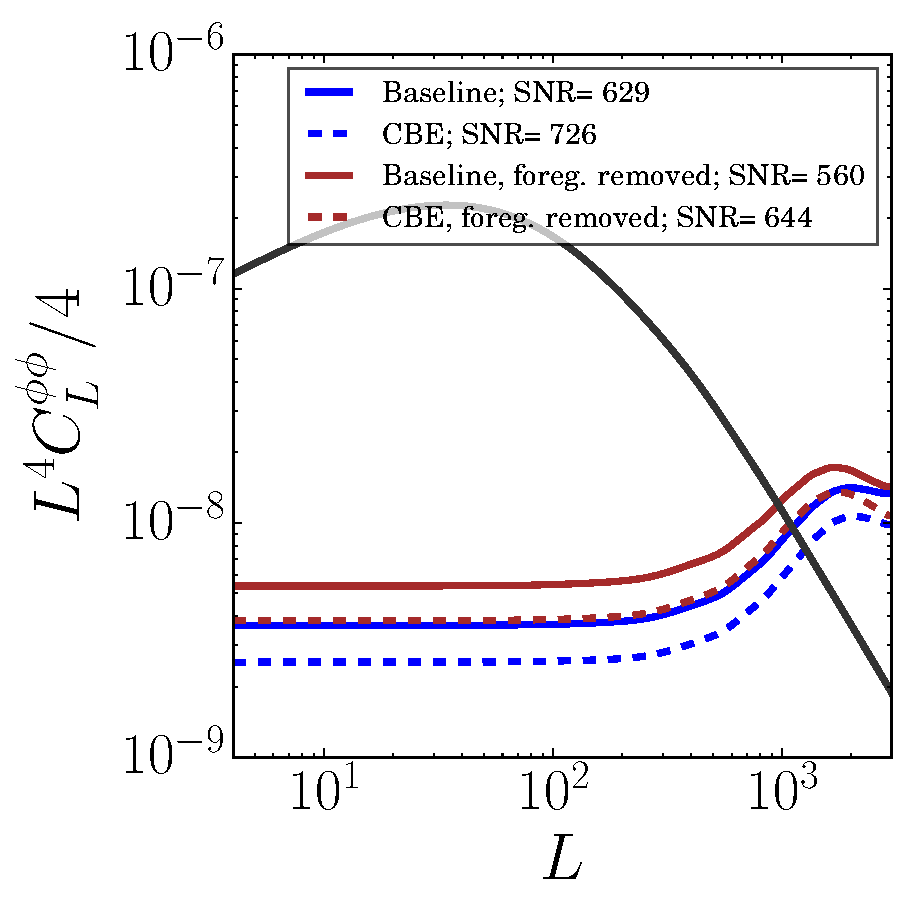
\includegraphics[width=2.5in]{images/lensingNoisePICO.pdf} } }
\hspace{0.in}
\parbox{3.3in}{
\caption{\captiontext 
Theoretically predicted lensing power spectrum $C_{L}^{\phi \phi}$ (black) and forecasted PICO noise levels, with (red), and without (blue) deprojection, i.e. removal, of foregrounds. PICO will make a map of $\phi$ at angular scales where the noise is below the signal.  
\label{fig:lensingNoisePICO} 
} }
\vspace{-0.1in}
\end{figure}

The value of the reconstructed lensing map is immense, as has already been demonstrated with the much lower \ac{SNR} map from \planck . The unprecedented constraints on neutrino mass, discussed on page~\pageref{neutrino_fundamental}, are a direct result of this deep map. Tomographic cross-correlations of the lensing map with wide-field samples of galaxies and quasars will yield constraints on structure formation. The measurements will constrain the properties of quasars and other high-redshift astrophysics, e.g., a precise determination of the quasar bias (and hence host halo mass) as a function of their properties, such as (non-)obscuration. The map will be cross-correlated with other large-scale tracers to probe fundamental physics.  For instance, one can use correlations between large-scale structure tracers with different clustering bias factors and measure the relative difference between their clustering power spectra to effectively cancel cosmic variance~\citep{2009PhRvL.102b1302S,2018PhRvD..97l3540S}; this can constrain physics that affects the biasing of objects on large scales, such as primordial local non-Gaussianity~\citep{2008PhRvD..77l3514D}.  In Fig.~\ref{fig:fnlconstraint} we show the expected constraints for the CMB lensing field as reconstructed with PICO, in cross-correlation with  three years of the LSST survey. It can be seen that depending on the minimal multipole that can be used in the cross correlation, which is uncertain in both LSST and the PICO lensing map, the well-motivated theory target of $\sigma (f_\mathrm{NL}) \simeq 1$ \citep{2014arXiv1412.4671A} can be within reach. Values of $f_\mathrm{NL}$ at or above this level are a generic prediction of multi-field inflationary models.

Using the same cross-correlation techniques, it is also possible to constrain the evolution of the amplitude of structure as a function of redshift.  Fig.~\ref{fig:sigma8constraint} shows constraints on the amplitude of linear structure in several redshift bins.  This is a model-independent representation of the structure growth constraints; these measurements will yield constraints on dark energy or modified gravity, in the context of specific models.  The measurements can also be used for a neutrino mass constraint that is complementary to and competitive with that inferred from the CMB lensing auto-power spectrum described earlier.  


\begin{figure}
\hspace{-0.in}
\parbox{3.1in}{\centerline {
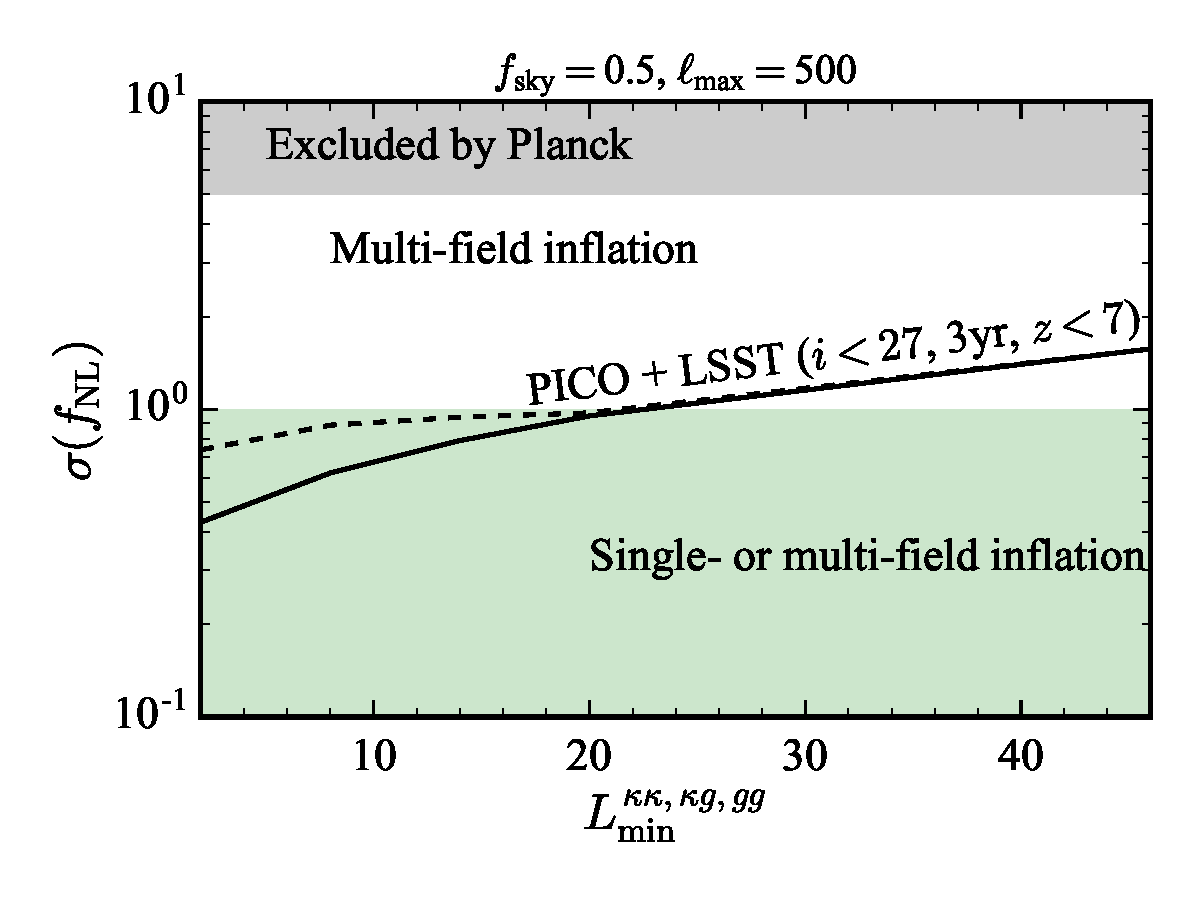
\includegraphics[width=2.7in]{images/PICO_fnl_lmin_PICOv4.1b_deproj0_SENS0.pdf} } }
\hspace{0.in}
\parbox{3.3in}{
\caption{\captiontext 
Forecasted sensitivity to  the parameter describing primordial non-Gaussianity of the local type for the PICO CMB lensing map together with three years of the LSST survey, as a function of the minimal multipole used in the analysis. A value of $\sigma (f_\mathrm{NL}) \simeq 1$ is a well-motivated theoretical target.  
\label{fig:fnlconstraint} 
} }
\vspace{-0.1in}
\end{figure}

%%  Fig. on left, caption on right  %%%%%%%%%%%%%%%%
%\begin{figure}
%\hspace{0.1in}
%\parbox{2.8in}{\centerline {
%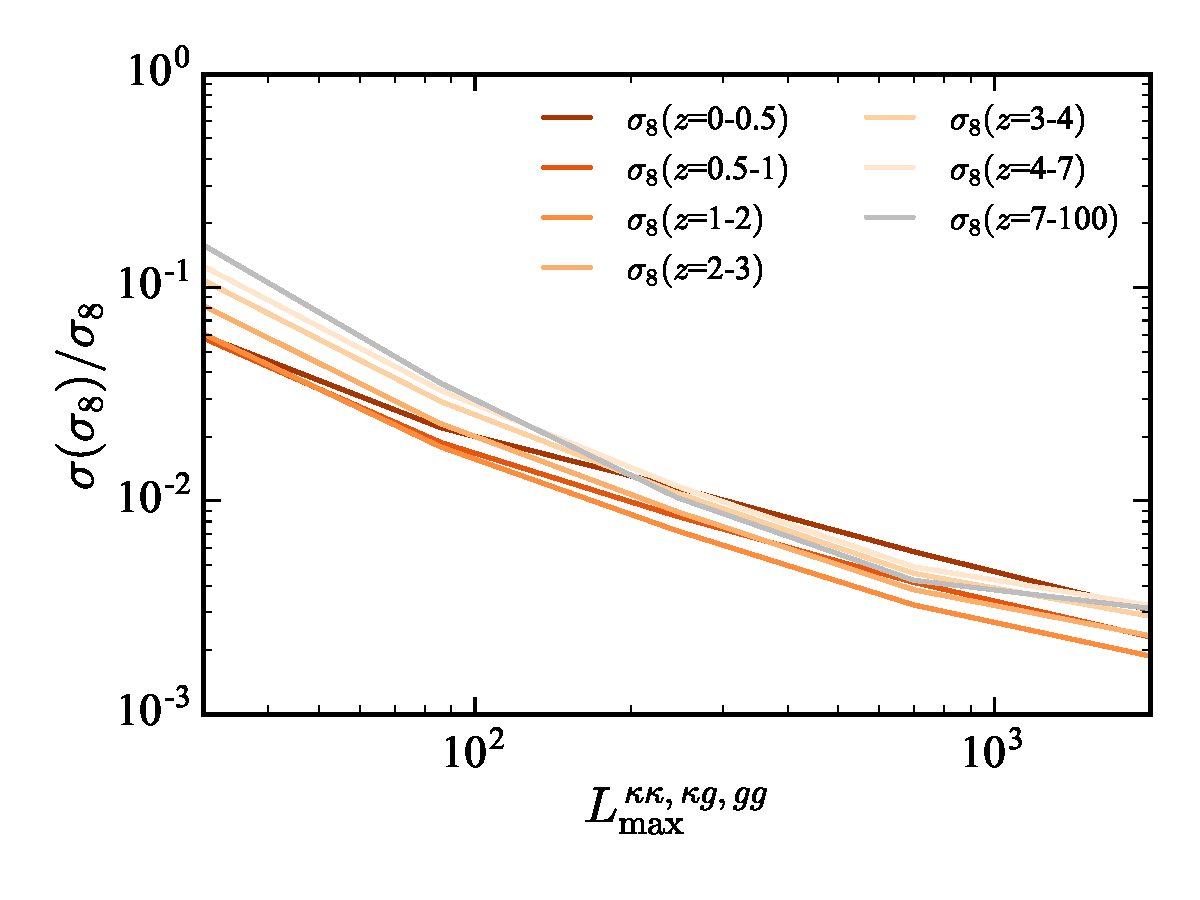
\includegraphics[width=2.5in]{images/PICO_s8_lmax_PICOv4.1b_deproj0_SENS0.pdf} } }
%\hspace{0.1in}
%\parbox{3.5in}{
%\caption{\captiontext\label{fig:sigma8constraint} Forecasted sensitivity to  the parameter describing the amplitude of structure in various redshift bins, as a function of the maximal multipole used in the analysis.  Percent-level constraints on these parameters allow for stringent tests of physics beyond $\Lambda$CDM that modify the rate of growth of structure. } }
%\vspace{-0.1in}
%\end{figure}

%% Fig. on right, caption on left  %%%%%%%%%%%%%%%%%%%%%%%%%%%
\begin{figure}
\hspace{0.1in}
\parbox{3.3in}{
\vspace{0.15in}
\caption{\captiontext  
Forecasted sensitivity to  the parameter describing the amplitude of structure in various redshift bins, as a function of the maximal multipole used in the analysis.  Percent-level constraints on these parameters allow for stringent tests of physics beyond $\Lambda$CDM that modify the rate of growth of structure. 
\label{fig:sigma8constraint} 
} }
\hspace{0.1in}
\parbox{2.9in}{\centerline {
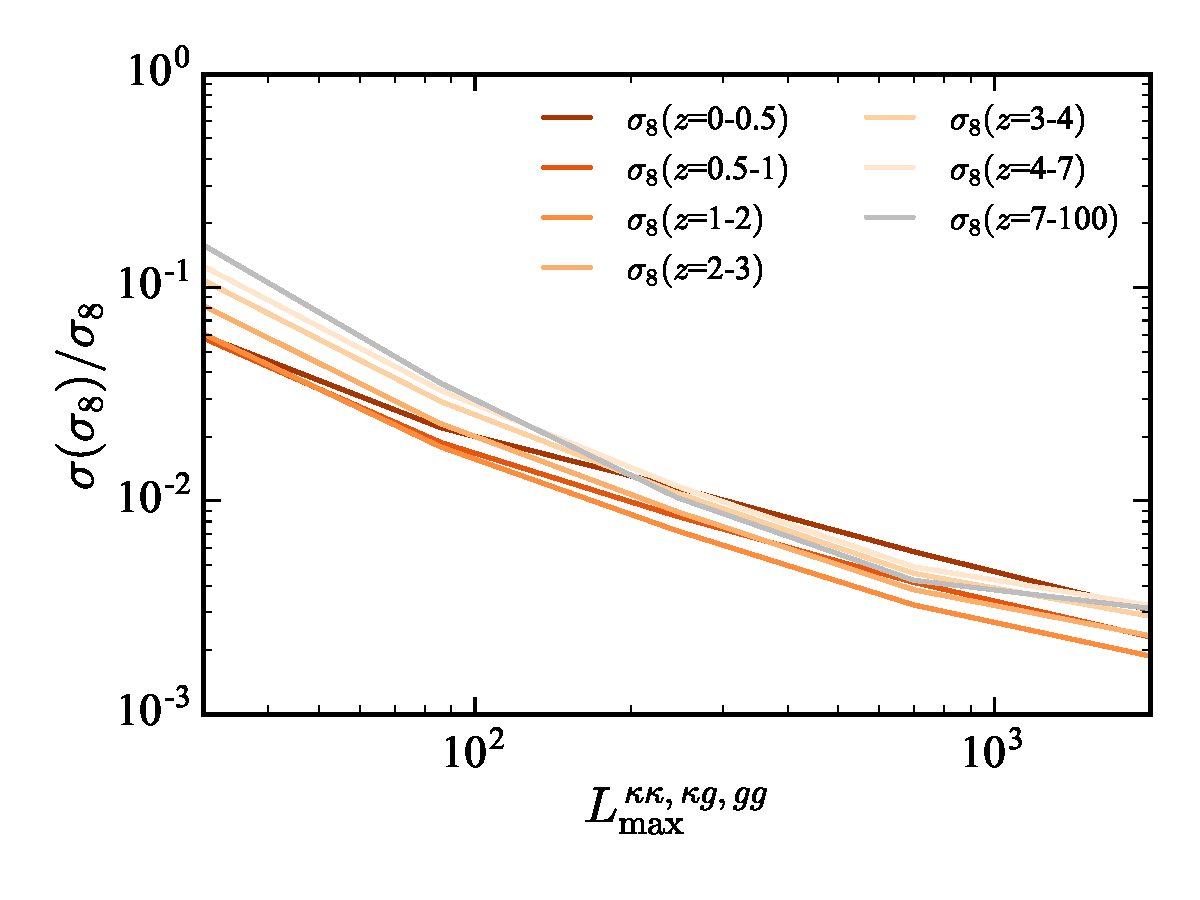
\includegraphics[width=2.6in]{images/PICO_s8_lmax_PICOv4.1b_deproj0_SENS0.pdf} } }
\vspace{-0.1in}
\end{figure}

%{\bf CMB halo lensing forecast (Jim, Jean-Baptiste)}

Lensing will also be used to weigh dark matter halos hosting galaxies, groups, and clusters of galaxies.  Calibrating the masses of galaxy clusters is the most uncertain and crucial step in the cluster cosmology program, in which CMB lensing has already begun to play an important role.  In this approach, known as CMB halo lensing, we focus on the small-scale effects of gravitational lensing around these objects~\citep{2015ApJ...806..247B, 2015PhRvL.114o1302M, 2016A&A...594A..24P}. The technique holds great potential for measuring halo masses out to high redshifts where gravitational lensing of galaxies (i.e., gravitational shear) no longer works because of the lack of background sources.

This is illustrated in Fig.~\ref{fig:HaloLensing}, which shows the mass sensitivity of PICO using a spatial filter optimized for extracting the mass of halos \citep{2015A&A...578A..21M}.  The curves give the $1\sigma$ noise in a mass measurement through the filter as a function of redshift. Their flattening at high redshift reflects the fact that CMB lensing is sensitive over a broad range of redshifts, extending well beyond the limit of $z=2$ shown in the figure.  We see that PICO can measure the mass of individual low-mass clusters ($\sim 10^{14}$\,M$_\odot$) over a wide redshift range, and by stacking we can determine the mean mass of much smaller halos, including those hosting individual galaxies.  

\begin{figure}[t]
\hspace{-0.1in}
\parbox{3.1in}{\centerline {
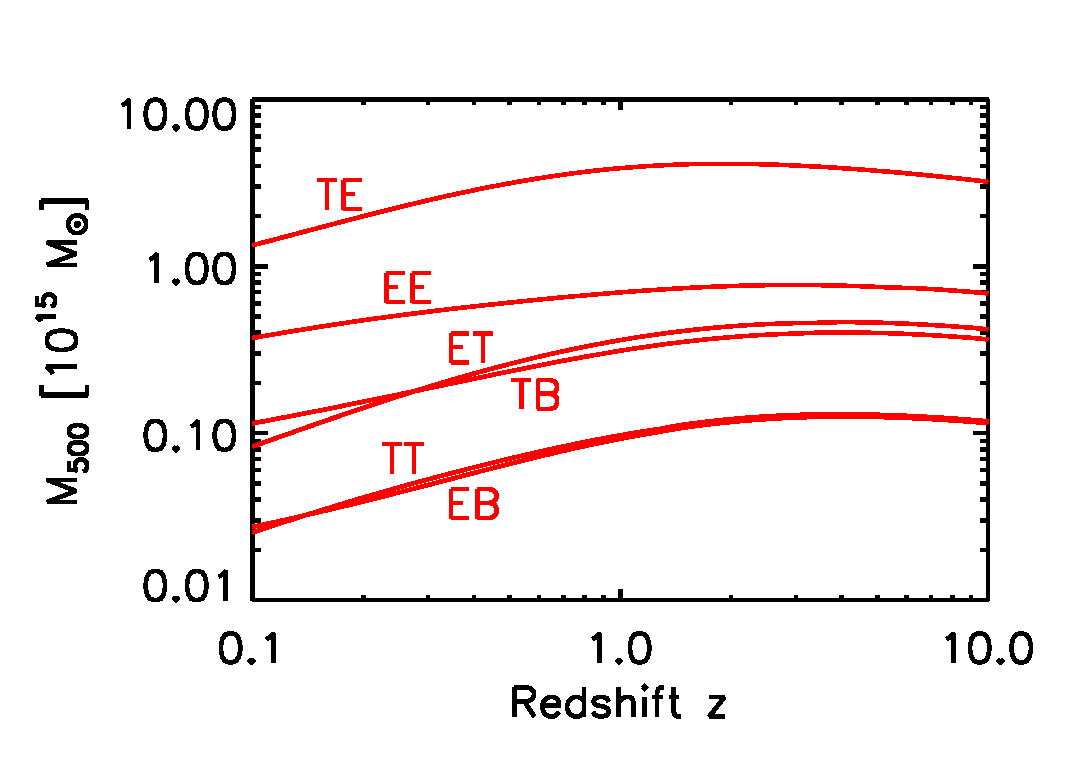
\includegraphics[width=3.0in]{images/m500lim_vs_z_pico_polar_v3.eps} } }
\hspace{0.in}
\parbox{3.4in}{
\caption{\captiontext 
PICO sensitivity for CMB halo lensing.  Curves for different CMB signal correlations give the $1\sigma$ sensitivity of an optimal mass filter \citep{2015A&A...578A..21M}.  The curves are flat at high redshift, demonstrating the essential property that CMB halo lensing can be probed over a very wide redshift range, and well beyond the $z=2$ limit of the figure.  For PICO, the $EB$ and $TT$ estimators are roughly equivalent, offering important cross-validation of measurements because the systematics are very different for temperature and polarization. 
\label{fig:HaloLensing} 
} }
\vspace{-0.1in}
\end{figure}

Halo lensing will enable calibration of the galaxy cluster mass scale, which is critical for our cosmological analysis of PICO cluster counts, as mentioned above.  It also gives a unique tool for measuring the relation between galaxies and their dark matter halos during the key epochs of cosmic star formation at $z\geq 2$, not reachable by other means.  This will provide valuable insight into the role of environment on galaxy formation during the rise to and fall from the peak of cosmic star formation at $z\sim 2$.  From a complementarity perspective, the high-resolution, high-frequency PICO channels will play an essential role in cleaning foregrounds for high-resolution ground-based halo lensing measurements at lower frequencies, particularly those derived from the temperature-based estimator, which is most contaminated by foregrounds. 
%
%%%%%%%%%%%%%%%%%%%%
%$\bullet$ {\bf Gravitational Lensing as Noise for Gravity Wave Science} \hspace{0.1in} \label{lensingnoise}
%\comor{does this belong here or in gravity waves?} One of the most pronounced effects of lensing is the emergence of the `lensing B-mode power spectrum', which is a result of gravitational lensing of $E$-modes into $B$-modes;  see Fig.~\ref{??}.  \comor{reference figure in fundamental physics?} When the tensor to scalar ratio $r \simeq 0.01$, the B-mode lensing power spectrum and the one from gravity waves have approximately the same level at $\ell = 80$, which is the angular scale at which the inflationary $BB$ spectrum peaks. For lower levels of $r$, this peak is masked by $E$-mode photons that are lensed into $B$. But the $B$-mode maps can be `delensed'~\citep{2004PhRvD..69d3005S,2012JCAP...06..014S}. The effect of lensing on $E$ and $B$ maps can be determined and undone if these maps are measured with few arcmin resolution and with sufficient depth. Forecasts for PICO show that at a minimum 73\% of the lens-induced $B$-mode power will be removed for the baseline configuration, after accounting for foreground subtraction. 80\% will be removed if the foregrounds do not degrade the inherent \ac{SNR}, rising to 85\% for the CBE configuration. Without delensing PICO determination of $r$ would be limited to $r>??$. We emphasize that PICO will be relying on its own data to conduct the delensing and foreground cleaning, thus avoiding reduced efficacy arising from the need to cross-calibrate experiments, identify common observing areas on the sky, not having frequency band coverage at the appropriate resolution to remove foregrounds, or from other systematic uncertainties.  \\
%
%%%%%%%%%%%%%%%%%%%%

\vspace{0.1in}
\noindent{\bf Constraining Galaxy Formation via the Sunyaev-Zel$^{\prime}$dovich (SZ) Effects} \hspace{0.1in} \label{sz}
Not all CMB photons propagate through the Universe freely; about 6\% are Thomson-scattered by free electrons in the intergalactic medium (IGM) and intracluster medium (ICM). These scattering events leave a measurable imprint on CMB temperature fluctuations, which thereby contain a wealth of information about the growth of structures and the thermodynamic history of baryons. A fraction of these photons are responsible for the thermal and kinetic Sunyaev--Zel$^{\prime}$dovich effects (tSZ and kSZ)~\citep{zeldovich69,SZ1972}. 
%The thermal SZ effect (tSZ) is the increase in energy of CMB photons due to scattering off hot electrons. This results in a spectral distortion
%, proportinal to the electron pressure,
% of the CMB blackbody that corresponds to a decrement in CMB temperature at frequencies below 217 GHz and an increment at frequencies above. The kSZ effect is the Doppler shift of CMB photons Thomson-scattering off free electrons that have a non-zero peculiar velocity with respect to the CMB rest frame. 
%This produces small shifts in the CMB temperature proportional to the radial velocity of the object and its optical depth.
The amplitudes of the tSZ and kSZ signals are proportional to the integrated electron pressure and momentum along the line of sight, respectively.  They thus contain information about the thermodynamic properties of the IGM and ICM, which are highly sensitive to astrophysical \lq{feedback}\rq. Feedback is the process of energy injection into the IGM and ICM from accreting supermassive black holes, supernovae, stellar winds, and other sources.
%since their magnitudes are proportional to the integrated electron pressure (tSZ) and momentum (kSZ) along the line of sight.
The tSZ effect will be used to measure ensemble statistics of galaxy clusters, which contain cosmological information, as well as to provide uniform cluster samples for galaxy-formation studies in dense environments. 

%
%\item Cosmological parameters from the abundance of tSZ-detected clusters and statistics of component-separated tSZ maps.
%\item Thermodynamic properties of galaxies, groups, and clusters from combined tSZ and kSZ cross-correlation measurements.
%\item Measurements of peculiar velocities, which are powerful cosmological probes on large scales, through the kSZ effect.
%\item Patchy reionization which imprints the CMB through higher order moments of the kSZ effect.
%%%%%%%%%%%%%%%%%%%%
\noindent$\bullet$ {\bf Galaxy Clusters} \hspace{0.1in} \label{clusters}  Galaxy clusters found via the tSZ  effect provide a well-defined sample with a selection function. That is simple to model. Such samples of clusters are straightforward to use for cosmological inference and studies of galaxy evolution in dense environments. The tSZ-selected sample from PICO will provide all clusters with masses above $\sim3\times10^{14} M_\odot$ (defined with respect to the radius within which the average density reaches 200 times the critical density) out to high redshifts, 
%\comor{which high redshift?}
as long as the clusters have started to virialize. We forecast that PICO will find $\sim$150,000 galaxy clusters, assuming the cosmological parameters from \planck\ and applying a foreground mask, using only 70\% of the sky. With redshifts provided by optical surveys and infrared follow-up observations, the PICO tSZ-selected cluster sample will be an excellent cosmological probe, with mass calibration provided by CMB halo lensing described above and optical weak lensing for clusters with $z < 1.5$. 
%\comor{why is it an excellent cosmological probe? didn't we want to add forecasts on parameters such as neutrino mass, and dark energy? wasn't there a point about a sample that is not restricted to a particular location in the sky?}

%\comor{Points to still hit
%High z sample,
%Numbers -- Nick and Jim should cross-check,
%most massive cluster all over the whole sky,
%Cosmology.}
%
%%%%%%%%%%%%%%%%%%%%
\noindent$\bullet$ {\bf Compton-$y$ map and tSZ auto-power spectrum} \hspace{0.1in} \label{ymap}  In addition to finding individual clusters, multifrequency CMB data also allow the reconstruction of full-sky maps of the tSZ signal. These are called  \lq Compton-$y$ maps\rq. %via foreground removal algorithms similar to those used to obtain cleaned maps of the CMB.  
With its extremely low noise and broad frequency coverage, which is essential for separating out other signals, PICO will yield a definitive Compton-$y$ map over the full sky, with high \ac{SNR} down to angular scales of a few arcminutes.  We quantify this expectation by reconstructing the Compton-$y$ field using the needlet internal linear combination (NILC) algorithm~\citep{Delabrouille2009} applied to sky simulations generated with the \planck~ sky model, with maps at all PICO frequencies (with appropriate noise added).  The error bars on the reconstructed tSZ power spectrum are shown in Fig.~\ref{fig:PICO_tSZ_PS}, in comparison to current measurements.  The total \ac{SNR} is 1270 for the PICO CBE configuration, with the PICO baseline configuration only $\approx 10$\% lower.  This is nearly two orders of magnitude higher \ac{SNR} than \planck , which has already provided data with much higher \ac{SNR} than ground-based experiments. 
\begin{figure}
\hspace{-0.1in}
\parbox{3.1in}{\centerline{
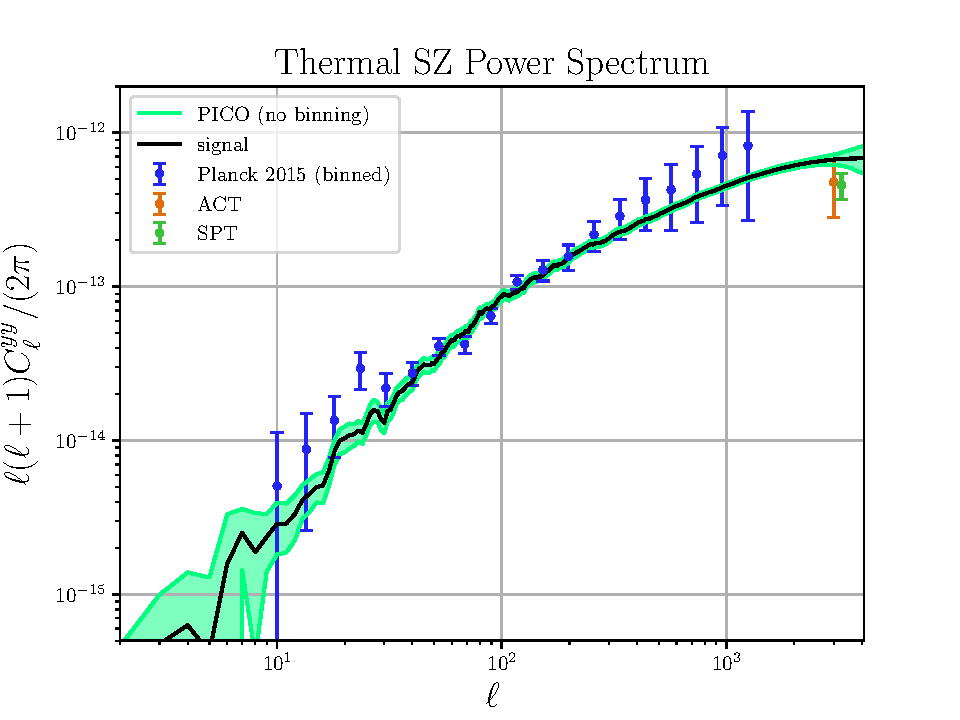
\includegraphics[width=3.0in]{images/PICO_tSZ_PS_plot.pdf} } }
\hspace{0.in}
\parbox{3.4in}{
\caption{\captiontext  
Constraints on the tSZ power spectrum from PICO and current data.  A simulated tSZ power spectrum (black) is constrained at each multipole by PICO's data ($1\sigma$, green). Binning in $\ell$, would increase the \ac{SNR} beyond the calculated value of 1270, which is already nearly 100 times larger than from \planck\ (blue). We include current measurements by the SPT and ACT, two ground-based programs~\citep{Sievers2013,George2015}
%The black curve shows the simulated tSZ power spectrum signal.  The light green shaded region shows the error bars for PICO at each multipole, i.e., with no binning, as determined from NILC analysis of full-sky simulations.  The blue points show the current constraints from Planck, which have been averaged into broad multipole bins.  The orange and dark green points show the constraints from ACT and SPT, respectively, at a single multipole of $\ell=3000$.  The overall PICO $S/N = 1270$, nearly two orders of magnitude larger than current measurements.
\label{fig:PICO_tSZ_PS} 
} }
\vspace{-0.1in}
\end{figure}

Extremely strong constraints on models of astrophysical feedback will be obtained from the analysis of the PICO $y$-map, both from its auto-power spectrum and from cross-correlations with galaxy, group, cluster, and quasar samples.  Like the CMB-lensing map described above, the legacy value of the PICO $y$-map will be immense.  As an example, we forecast the detection of cross-correlations between the PICO $y$-map and galaxy weak lensing maps constructed from LSST and WFIRST data.  Considering the LSST \lq gold\rq~sample with a source density of 26 galaxies/arcmin${}^2$ covering 40\% of the sky, we forecast a detection of the tSZ-weak lensing cross-correlation with \ac{SNR} = 3000.  Cross-correlations with the galaxies themselves will be measured at even higher \ac{SNR}.  At this immense significance, the signal can be broken down into dozens of tomographic redshift bins, yielding a precise tracing of the evolution of thermal pressure over cosmic time.  For PICO and WFIRST (assuming 45 galaxies/arcmin${}^2$ covering 5.3\% of the sky), we forecast \ac{SNR} = 1100 for the tSZ-weak lensing cross-correlation.  The WFIRST galaxy sample extends to higher redshift, and thus this high-\ac{SNR} measurement will allow the evolution of the thermal gas pressure to be probed to $z \approx 2$ (the peak of the cosmic star formation history) and beyond.  These transformative measurements will revolutionize our understanding of galaxy formation and evolution by distinguishing between models of feedback energy injection at high significance.  Additional cross-correlations of the PICO $y$-map with quasar samples, filament catalogs, and other large-scale structure tracers will provide valuable information on baryonic physics that is complementary to inferences from the lensing cross-correlations described earlier. %\comor{is this already covered earlier in Marcel's lensing cross-correlations text?}



\end{document}


%Measurements of the CMB reveal structure imprinted not only at the early time of recombination, but also at nearly every significant ensuing epoch in cosmic history.  In particular the matter between us and the CMB last-scattering surface will deflect the path of CMB photons, a process known as gravitational lensing.  Although the lensing of the CMB is a weak signal, targeted statistical estimators enable its extraction.  Measurements of the lensing signal have rapidly progressed, from the first detections in 2007-8 \citep{2007PhRvD..76d3510S, 2008PhRvD..78d3520H} to the recent $40\sigma$ measurement by the {\it Planck} team \cite{2018arXiv180706210P}.  When applied to a rich dataset such as that expected from the PICO satellite, these estimators will provide a map of all the matter in the Universe in projection, with the most sensitivity at redshift $z \simeq 2$ and down to scales of approximately ten arcminutes.  

%Forecasts show that the power spectrum of lensing in the PICO CMB map can be detected at approximately 580$\sigma$ or 650$\sigma$ for the requirement or CBE configurations, respectively.  Such high-S/N measurements are more than an order of magnitude improvement over the current state of the art, obtained by the {\it Planck} team.  The legacy value of the PICO CMB lensing map is immense, as has already been seen with {\it Planck}, particularly through the high-S/N cross-correlation science that will be enabled.  For example, tomographic cross-correlations of the PICO CMB lensing map with samples of galaxies and quasars will yield constraints on structure formation out to redshifts inaccessible to galaxy surveys or galaxy weak lensing maps on their own.  These measurements will yield constraints on dark energy, modified gravity, and neutrino mass (complementary to the neutrino mass inferred from the CMB lensing auto-power spectrum described earlier).  In addition, PICO CMB lensing cross-correlations will yield constraints on the properties of quasars and other high-redshift astrophysics, e.g., a precise determination of the quasar bias (and hence host halo mass) as a function of their properties, such as (non-)obscuration.  We provide further quantitative cross-correlation forecasts below.  Fig.~\ref{fig:lensingNoisePICO} shows per-mode noise curves for the reconstruction of CMB lensing from PICO, demonstrating the wide range of angular scales over which the matter density field will be mapped.  \textbf{Add brief discussion of foreground robustness demonstrated in Fig.~\ref{fig:lensingNoisePICO}}

%\begin{figure}[!htb]
%\centering
%
\includegraphics[width=4cm]{images/example}
%\caption{example}
%\label{fig:im_3}
%\end{figure}
